\documentclass{article}
\usepackage{amsmath,amsthm,amsfonts,microtype,amssymb}
\usepackage{enumitem}
\usepackage{parskip}
\usepackage{mathpazo}
\usepackage{tikz-cd}
\usepackage{geometry}
    \geometry{top=1in}
\usepackage{graphicx}
\usepackage{float}


\usepackage{hyperref}
    \hypersetup{%
        colorlinks=true,
        linkcolor=red,
        filecolor=red,      
        urlcolor=red,
        bookmarks=true,
        pdfpagemode=FullScreen,
    }

\newtheorem{theorem}{Theorem}


\title{Homework 03 \\ Computations using the Seifert--van Kampen Theorem}
\author{Algebraic Topology - Winter 2021}
\date{Due: \textbf{February 04, 2021, 11:59 pm}}

\begin{document}
\pagenumbering{gobble}
\maketitle

    % \item Let $(X,x)$ and $(Y,y)$ be connected spaces in $\mathbf{Top}_*$ which are not contractible. Recall that the \emph{wedge product} is defined as 
    % \begin{align*}
    %     X \vee Y := \left( X \coprod Y \right)/ (x \sim y).
    % \end{align*}
    % Find some sufficient condition(s) for the following statement to be true:
    % \begin{align*}
    %     \pi_1(X \vee Y) \cong \pi_1(X) * \pi_1(Y).
    % \end{align*}
\begin{enumerate}
    \item Let $X$ be a non-empty space in $\mathbf{Top}$.
    \begin{enumerate}
    \item We defined the cone over $X$ as
        \begin{align*}
            \mathrm{cone}(X) := X \times [0,1] / (x,1) \sim (x',1)
        \end{align*}
        for all $x, x' \in X$.
        Show that $\mathrm{cone}(X)$ is contractible.
    \item 
    We defined the suspension of $X$ as 
    \begin{align*}
        SX := X \times [-1,1] / ((x,-1) \sim (x',-1) , (x,1) \sim (x',1))
    \end{align*}
    for all $x,x' \in X$. Show that $SX$ is path-connected.
        \item Show that if $X$ is path-connected then $SX$ is simply-connected.
        \item Show that $S^{n+1} \cong S(S^n)$, where $S^n$ is the $n$ dimensional sphere
        \begin{align*}
            S^n = \{ (x_0, x_1, \dots, x_n) \in \mathbb{R}^{n+1} : x_0^2 + x_1^2 + \dots + x_n^2 = 1\}.
        \end{align*}
        \item Conclude that $S^n$ is simply-connected for $n > 1$.
    \end{enumerate}

    \item 
    Let $A, X$ be path-connected spaces in $\mathbf{Top}$ and let $i: A \to X$ be a continuous map between them.
    Define the mapping cone of $i$ as 
    \begin{align*}
        \mathrm{cone}(i) := A \times [0,1] \sqcup X / ((a,1) \sim (a',1), (a,0) \sim i(a))
    \end{align*}
    \begin{figure}[H]
        \centering          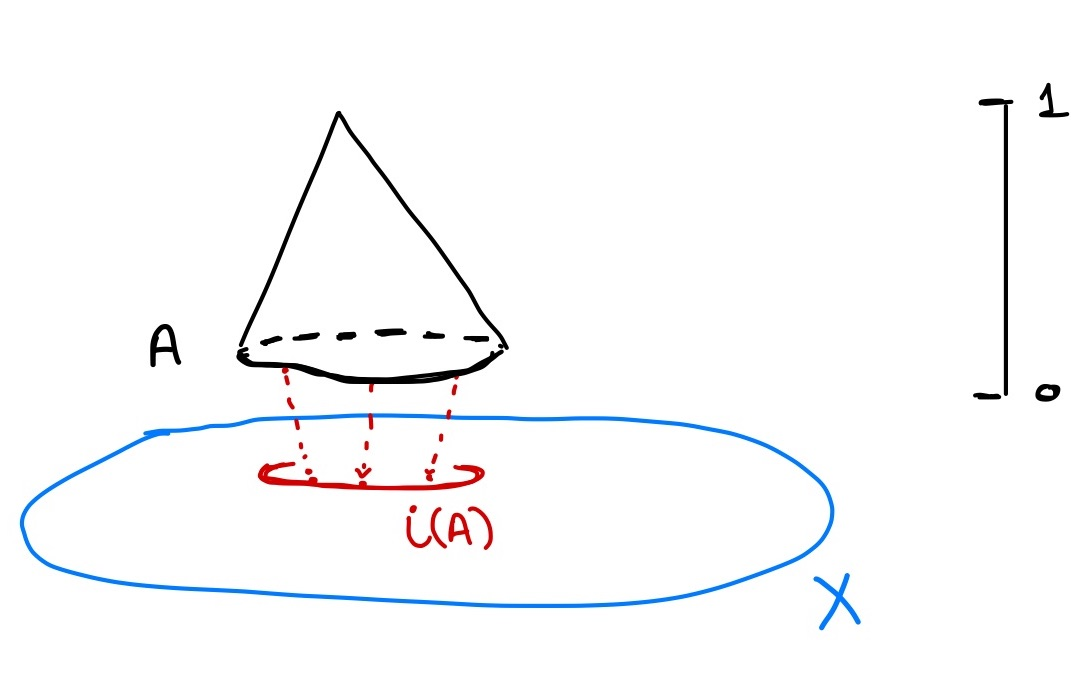
\includegraphics[height=5cm]{images/mapping cone.jpg} 
    \end{figure}
    Compute $\pi_1(\mathrm{cone}(i))$ in terms of $\pi_1(A)$, $\pi_1(X)$, and $\pi_1(i)$.
    In the special case when $i$ is an inclusion of CW complexes, one can show that $\mathrm{cone}(i) \simeq X/A$. This gives us a way to compute $\pi_1(X/A)$ for CW complexes.
    \end{enumerate}
    You do not have to provide completely rigorous proofs for the following question.
    For all the technical details see Hatcher, Pg. 50.
    \begin{enumerate}[resume]
    \item 
    Let $X$ be a path-connected CW complex with a finite number of cells. 
    Let $\{\mathbb{D}^n_\alpha\}_{\alpha \in \mathrm{cell}(n)}$ be the set of $n$-cells of $X$.
    Let $\mathrm{gl}_\alpha^n : \partial \mathbb{D}_\alpha^n \to X^{n-1}$ be the gluing maps, where $X^{n-1}$ is the ${(n-1)}^{th}$ skeleton of $X$.
    \begin{enumerate}
        \item Argue that the space obtained by attaching a single cell $\mathbb{D}_\alpha^n$ to $X^{n-1}$ using the gluing map 
        $\mathrm{gl}_\alpha^n : \partial \mathbb{D}_\alpha^n \to X^{n-1}$
        is homeomorphic to $\mathrm{cone}(\mathrm{gl}_\alpha^n)$.
        \end{enumerate}
        Thus CW complexes are essentially sequences of mapping cones.
        Use your answers for Q.1 and Q.2 to prove the following.
        \begin{enumerate}[resume]
        \item 
        The map $\pi_1(X^2) \to \pi_1(X)$ induced by the inclusion of the 2-skeleton is an isomorphism.
        
        \item The map $\pi_1(X^1) \to \pi_1(X^2)$, induced by the inclusion $X^1 \hookrightarrow X^2$, is a surjection.
        \item The kernel of the above map is the normal subgroup generated by the elements  $\pi_1(\mathrm{gl}^2_\alpha)\left([\gamma_\alpha]\right)$ where $\alpha \in \mathrm{cell}_2(X)$ and $[\gamma_\alpha]$ is the generator of $\pi_1(\partial \mathbb{D}^2_\alpha)$.
    \end{enumerate}
    Thus the 1-skeleton gives us the generators and the 2-cells give us the relations of $\pi_1(X)$.
    
    \item 
    \begin{enumerate}
        \item Compute the fundamental group of a genus 2 surface by applying the Seifert--van Kampen to the following open sets:
        \begin{figure}[H]
            \centering          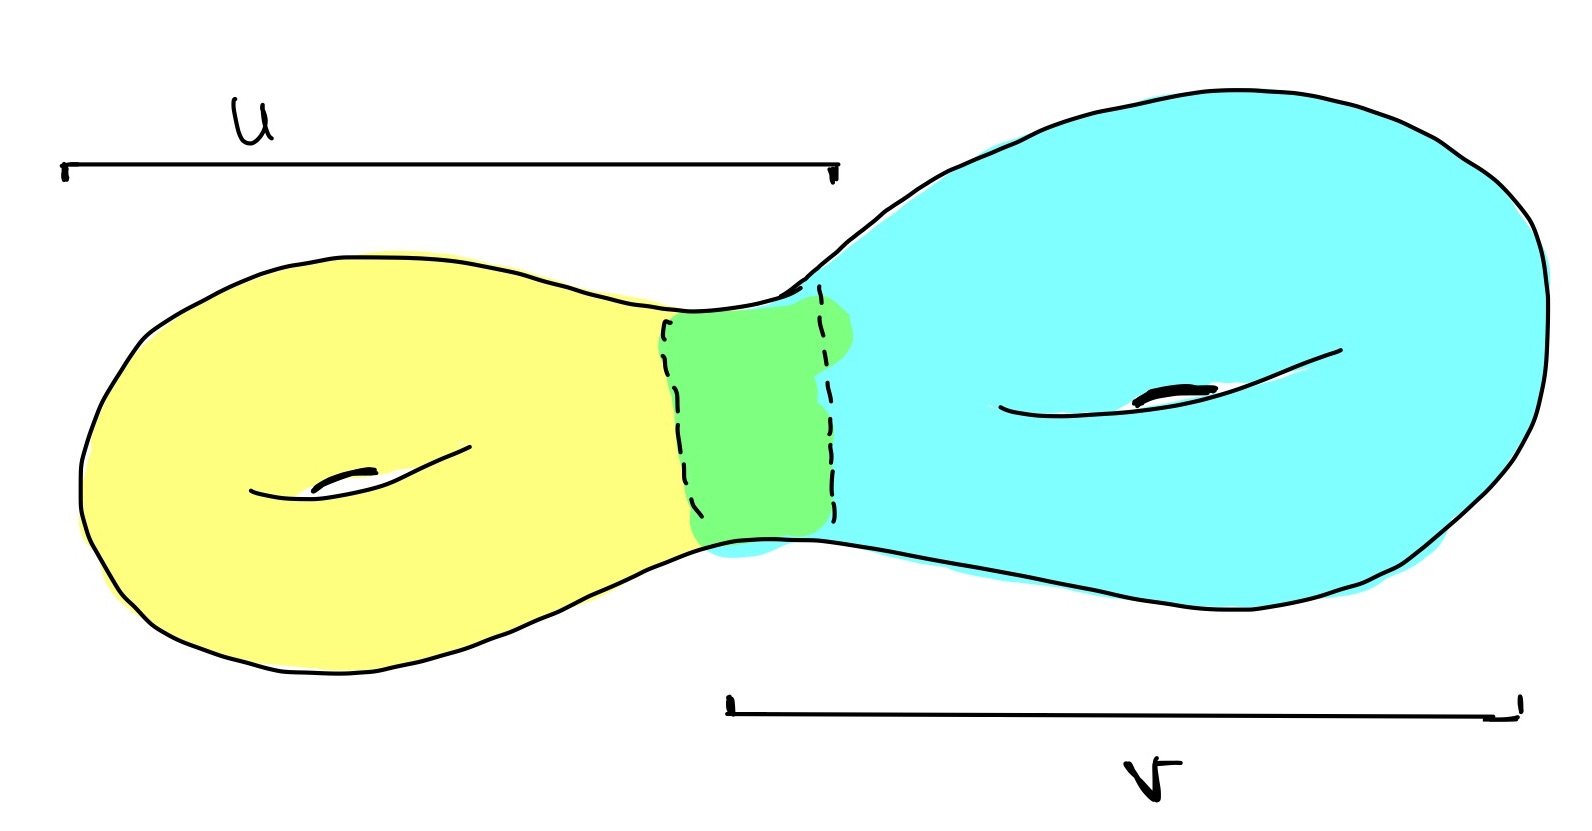
\includegraphics[height=4cm]{images/genus2-seifert-van-kampen.jpg} 
        \end{figure}
        
        \item Compute the fundamental group of genus $g$ surfaces using gluing diagrams.

        % \item Use the gluing diagrams given on the last page here: \url{https://mathcircle.berkeley.edu/sites/default/files/archivedocs/2010_2011/lectures/1011lecturespdf/bmc_topology_manifolds.pdf} to compute the fundamental group of the Klein bottle and the real projective space $\mathbb{RP}^2$.
    \end{enumerate}
    It is highly non-trivial to determine directly the isomorphism classes of these fundamental groups (give it a try!). One trick is to instead study their abelianizations $\pi_1(X)/[\pi_1(X), \pi_1(X)]$.\footnote{We'll later on show that abelianization of the fundamental group is isomorphic to the first homology group.}
    \begin{enumerate}[resume]
        \item Compute $\pi_1(X)/[\pi_1(X), \pi_1(X)]$ for the various spheres and genus $g$ surfaces.
        \item What can you say about homeomorphisms between the various spheres and genus $g$ surfaces using just $\pi_1(X)/[\pi_1(X), \pi_1(X)]$?
    \end{enumerate}
    
\end{enumerate}


\section*{Suggested exercises for practice from Hatcher}

\begin{description}
    \item[Pg. 19] 19, 21, 22
    \item[Pg. 53] 3, 4, 5, 7, 8, 9, 11
\end{description}

% \begin{enumerate}
%     \item (Optional exercise to try if you are comfortable with pushouts)
% \begin{enumerate}
%         \item Let $(X,x)$ be a space in $\mathbf{Top}_*$ and let $U$ and $V$ be open subsets of $X$ such that $x \in U \cap V$.
%         Show that the pushout of the inclusions $j_U: U \cap V \to U$ and $j_V:U \cap V \to V$ in $\mathbf{Top}_*$ is $U \cup V$.
%         % \begin{center}
%         % \begin{tikzcd}
%         %     U \cap V \arrow["j_U", r] \arrow["j_V", d, swap]  
%         %         & U  \arrow["i_U", d] \arrow["\varphi", ddr, bend left] \\
%         %     V \arrow["i_V", r, swap] \arrow["\psi", drr, bend right, swap]
%         %         & U \cup V \arrow["\exists !", dr, dashed] \\
%         %     & & Y.
%         % \end{tikzcd}
%         % \end{center}
%         \item Let $A, B, C$ be groups. Show that the pushout of group homomorphisms  $f: A \to B$ and $g : A \to C$ in $\mathbf{Groups}$ is $B * C / N$ , where $N$ is the smallest normal subgroup of $B *C$ generated by the elements $f(a)^{-1} g(a)$ for all $a \in A$.
%         % \begin{center}
%         % \begin{tikzcd}
%         %     A \arrow["f", r] \arrow["g", d, swap]  
%         %         & B  \arrow["f'", d] \arrow["f''", ddr, bend left] \\
%         %     C \arrow["g'", r, swap] \arrow["g''", drr, bend right, swap]
%         %         & B * C / N \arrow["\exists ! u", dr, dashed] \\
%         %     & & D''.
%         % \end{tikzcd}
%         % \end{center}    
%     \end{enumerate}
%     Thus the Seifert--van Kampen theorem says that $\pi_1: \mathbf{Top}_* \to \mathbf{Groups}$ preserves certain kinds of pushouts.\footnote{See also \url{https://math.stackexchange.com/questions/985606/what-categorical-limits-and-colimits-does-pi-1-preserve}.}
% \end{enumerate}

\end{document}
